\documentclass[a4paper]{report}

% do not ignore non-ascii chars
\usepackage{fontspec}

% use harvard-style referencing
\usepackage[round]{natbib}
\renewcommand{\bibname}{References}
\bibliographystyle{abbrvnat}

% needed for URLs
\usepackage[hidelinks]{hyperref}

% beautiful tables
\usepackage{booktabs}

% set the font size of captions
\usepackage[font=small]{caption}

% package for drawing graphs
% source: http://www.texample.net/tikz/examples/simple-flow-chart/
\usepackage{tikz}
\usetikzlibrary{shapes,arrows}

\tikzstyle{block} = [rectangle, draw, fill=teal!20, text centered, rounded corners, minimum height=0.9cm, node distance=1.6cm]
\tikzstyle{line} = [draw, -latex']


\begin{document}

\title{IPA alignment using vector representations}
\author{Pavel Sofroniev, Çağri Çöltekin (advisor)}
\date{March 2018}
\maketitle

\begin{abstract}
	This paper compares various methods of aligning IPA-encoded sound sequences using vector representations of phonemes.
\end{abstract}


\chapter{Introduction}

Most of the computational methods developed in the field of historical linguistics involve the task of aligning sound sequences,
either on its own or as a necessary step in a larger application.
In its essence, sequence alignment is a way to arrange two or more sequences together
in order to identify sub-sequences which are similar according to certain pre-defined criteria.
Usually in the context of historical linguistics these are sequences of phonological or phonetic segments comprising transcriptions of words;
and the similarity of given segments is subsequently used to infer either the cognacy of these words or rules of sound correspondences.

The standard algorithm for pairwise (i.e. aligning two sequences at a time) alignment
was originally developed by \citet{1970_Needleman_Wunsch} for aligning amino acid sequences.
Given a function that assigns scores to pairs of sequence elements,
the Needleman-Wunsch algorithm is guaranteed to find the alignment(s) that minimises/maximises the overall score.
There exist a number of variants of the basic algorithm, e.g. \citet{1981_Smith_Waterman},
and many of these have been adapted for the purposes of computational linguistics;
however, the output always depends to a great extent on the scoring function.
Some of these variants have been developed for aligning more than two sequences at once,
e.g. the T-Coffee algorithm by \citet{2000_Notredame_al}, but in this paper we focus on pairwise alignment only.

Unlike in bioinformatics, which deals primarily with sequences composed out of small sets of well-defined units,
in historical linguistics the encoding of sequences posed for alignment is not a solved problem.
Even though in general the standard way to encode sound sequences is IPA, the International Phonetic Alphabet,
for the purposes of alignment the overwhelming diversity of sound segments impedes the creation of a useful scoring function.
That is why modern sound sequence alignment methods tend to operate on small sets of segments;
IPA-encoded data is handled by translating it into the respective reduced alphabet.
While this constitutes a valid approach to tackle the problem of deriving a scoring function for the rich set of IPA segments,
in this paper we experiment with an alternative approach: vectorisation.
The goal is to obtain representations of IPA segments in a vector space
in which the cosine similarity between segments' vectors would reflect the segments' similarity and, hence, probability of shared ancestry.

Our inspiration for experimenting with vector representations (also known as embeddings)
is drawn from the success of such methods in other fields of computational linguistics:
e.g. \citet{2013_Mikolov_al} affirm that vector representations of words exhibit useful semantic and syntactic properties;
and \citet{2014_Chen_Manning} use word embeddings for transition-based parsing.
More closely related to our topic,
\citet{2018_Silfverberg_al} obtain vector representations of orthographic segments for Finnish, Spanish and Turkish
from recurrent neural networks trained to perform an inflection task.


\section{Background}

This section provides a concise overview of sound sequence alignment methods reported in the computational historical linguistics literature.


\subsection{Early methods}

An early method for sound sequence alignment reported in the literature is the one proposed by \citet{1996_Covington},
which was subsequently improved and extended in \citet{1998_Covington}.
Although the method does not take advantage of any standard sequence alignment algorithm and instead performs branch-and-bound search,
it does use a scoring function.
This function assigns hand-crafted values depending on whether the segments are consonants, vowels, or glides.
Due to this simple classification, the method could be adapted to work with IPA sequences (the author uses an undocumented encoding);
however, the better performance of more complex class-based methods have shown that such coarse three-way classification is not sufficient.

ALINE, first introduced by \citet{2000_Kondrak} and further elaborated in \citet{2002_Kondrak_Hirst} and \citet{2003_Kondrak},
employs a complex scoring function that is built around multi-valued (e.g. manner of articulation) and binary (e.g. nasality) phonetic features,
each with its relative weight, as well as some additional parameters (e.g. relative weight of vowels).
While some of these numerical values have been determined based on observations from the field of articulatory phonetics,
others have been established by trial and error.


\subsection{ASJP}

The Automated Similarity Judgement Program (ASJP) is an actively developed database aiming to provide
the translations of a set of 40 basic concepts into all the world's languages.
At the time of writing the database covers 294\,548 words from 7221 languages \citep{2016_Wichmann_al}.
The words are encoded using a uniform transcription consisting of 34 consonants and 7 vowels,
originally introduced by \citet{2008_Brown_al} as ASJPcode but now commonly known as ASJP.
This restricted set of encoding symbols results in much of the phonetic information being lost,
but the authors argue that such information might not be that valuable for certain applications.
The simplified encoding also allows for a greater reach of the database as many of the world's languages lack sufficiently detailed phonetic record.

\citet{2013_Jäger} uses the ASJP database to calculate the partial mutual information (PMI) scores\,---\,a logarithmic measure
for sound similarity based on occurrence and co-occurrence of the sound segments in data\,---\,for each pair of ASJP segments.
These PMI scores are successfully employed for inferring phylogenetic trees through determining language distances from PMI-based sequence alignment.
Unlike the aforementioned methods, this one obtains its scoring function in a data-driven manner, an approach also embraced in our paper.

PMI-based scoring has been used on IPA-encoded datasets as well, by converting the sequences to ASJP as a pre-processing step.
As an example, \citet{2016_Jäger_Sofroniev} use this approach to train a support vector machine (SVM) for cognate classification.


\subsection{Other methods}

The sound-class-based phonetic alignment (SCA) method developed by \citet{2012_List} employs a set of 28 sound classes.
It operates on IPA sequences by converting the segments into their respective sound classes, aligning the sound class tokens, and then converting these back into IPA.
The scoring function is hand-crafted to reflect the perceived probabilities of sound change transforming a segment of one class into a segment of another.


\chapter{Methods}

We consider 5 different methods for obtaining vector representations of IPA segments.
The code implementation of these methods, as well as of the experiments described in the next chapter,
is open sourced under the GNU GPLv3 license and publicly available online.\footnote{\url{https://github.com/pavelsof/ipavec}}
It is written using the Python programming language and a set of common dependencies, including NumPy, SciPy, scikit-learn, Gensim, and Keras.


\section{One-hot encoding}

Under one-hot encoding, given a vocabulary of $N$ distinct segments, each segment would be represented as a distinct binary vector of size $N$,
such that exactly one of its dimensions has value 1 and all its other dimensions have value 0.
In such a vector space, all vectors have length 1 and any two non-identical vectors are orthogonal.

One-hot encoding is a simple method, both conceptually and computationally, but it cannot be very useful for producing distance measures
because under its model each segment is equidistant from all the others.
For the purposes of this study one-hot vector representations are used as a baseline for comparing other methods.


\section{PHOIBLE feature vectors}

PHOIBLE Online is an ongoing project aiming to compile a comprehensive tertiary database of the world languages' phonological inventories.
At the time of writing the database contains phonological inventories for 1672 distinct languages making use of 2160 distinct IPA segments \citep{2014_Moran_al}.

As part of the project the developers are also maintaining a table of phonological features,
effectively mapping each segment encountered in the database to a unique ternary feature vector
(values indicate either the presence, absence, or non-applicability of the respective feature).
The feature table includes 39 distinct features and is based on research by \citet{2009_Bruce} and \citet{2011_Moisik_al}.
Table~\ref{tab:phoible-features} lists these, grouped by value, for an arbitrary segment.

\begin{table}[h]
	\centering\small
	\begin{tabular}{l *{3}{p{3.3cm}}}
		\toprule
		& present & absent & not applicable \\
		\midrule
		ə &
		syllabic, sonorant, continuant, approximant, dorsal, periodic glottal source &
		stress, short, long, consonantal, tap, trill, nasal, lateral, labial, coronal, high, low, front, back, tense,
		retracted tongue root, advanced tongue root, epilaryngeal source, spread glottis, constricted glottis, raised larynx ejective, lowered larynx implosive &
		tone, delayed release, round, labiodental, anterior, distributed, strident, fortis, click \\
		\bottomrule
	\end{tabular}
	\caption{The PHOIBLE features grouped by value for the segment ə}
	\label{tab:phoible-features}
\end{table}

The PHOIBLE feature vectors comprise segment representations grounded in phonology and linguistics theory
that could be readily used for a variety of computational endeavours.
Nevertheless, cosine distances in the vector space defined by the PHOIBLE features is equally affected by both common and rare features/dimensions;
for example the presence of a feature such as advanced tongue root in one of a pair of vectors
could result in a distance larger than needed for the purposes of alignment.
That is why we have also experimented with reducing the number of dimensions by applying principal component analysis (PCA),
expecting that this would decrease the influence of rare features; we refer to this method as PHOIBLE-PC.


\section{phon2vec embeddings}

The first data-driven method we consider is word2vec, first introduced by \citet{2013_Mikolov_al}.
It comprises two closely related model architectures for computing vector representations of words:
the continuous bag-of-words model (CBOW) which tries to predict a word based on its context of neighbouring words,
and the continuous skip-gram model which, given a word, tries to predict words from its context.
The resulting embeddings also depend on a few other parameters,
e.g. the number of neighbouring words that constitute a word's context, or the number of negative samples for each positive sample.

As our study concerns IPA segments rather than words, we refer to the method as phon2vec.
Our embeddings are trained on a dataset of tokenised IPA sequences,
with the model effectively treating the IPA segments as words and the sequences as sentences.


\section{NN embeddings}

Our fourth method consists of using the embeddings of a neural network (NN) which is trained to predict an IPA segment's immediate neighbours.
As it is the case with the phon2vec model, such a network requires a training dataset of IPA sequences.
During training, each IPA segment of each sequence is embedded, processed by a regular dense layer,
and used to predict the segment's one-hot encoded preceding and following segments through two softmax layers.
The network's architecture is depicted in Figure~\ref{fig:nn}.

\begin{figure}[h]
	\centering\small

	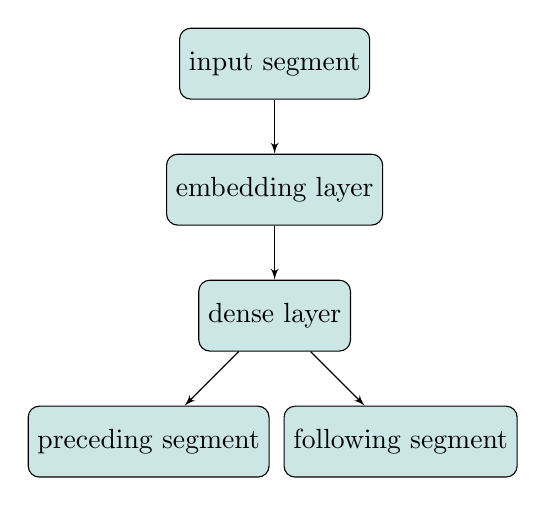
\begin{tikzpicture}
		\node [block] (input) {input segment};
		\node [block, below of=input] (embedding) {embedding layer};
		\node [block, below of=embedding] (dense) {dense layer};
		\node [block, below of=dense, left of=dense] (prev) {preceding segment};
		\node [block, below of=dense, right of=dense] (next) {following segment};

		\path [line] (input) -- (embedding);
		\path [line] (embedding) -- (dense);
		\path [line] (dense) -- (prev);
		\path [line] (dense) -- (next);
	\end{tikzpicture}

	\caption{NN: layers}
	\label{fig:nn}
\end{figure}


\section{RNN embeddings}

Our last method consists of using the embeddings of a recursive neural network (RNN).
Given a pair of sequences, the network recursively encodes the first sequence into a vector which is then recursively decoded into an output sequence.
The backward propagation of the mismatches between the output sequence and the pair's second sequence affects the whole network.
Introduced by \citet{2014_Cho_al}, networks of such architecture are typically employed for machine translation,
but our network is trained on pairs of IPA sequences comprising bilingual pairs of words linked to the same meaning.
As both encoded and decoded data are of the same form, the embedding layer is shared.
The network's architecture is depicted in Figure~\ref{fig:rnn}.

\begin{figure}[h]
	\centering\small

	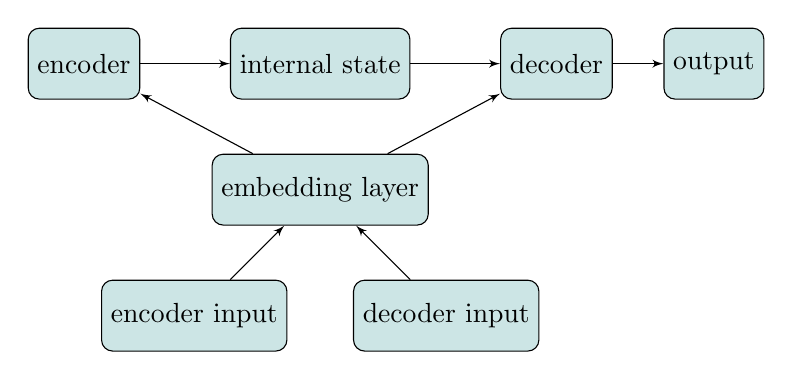
\begin{tikzpicture}
		\node [block] (encoder) {encoder};
		\node [block, right of=encoder, node distance=3cm] (state) {internal state};
		\node [block, right of=state, node distance=3cm] (decoder) {decoder};
		\node [block, right of=decoder, node distance=2cm] (output) {output};
		\node [block, below of=state] (embedding) {embedding layer};
		\node [block, below of=embedding, left of=embedding] (encoder-input) {encoder input};
		\node [block, below of=embedding, right of=embedding] (decoder-input) {decoder input};

		\path [line] (encoder-input) -- (embedding);
		\path [line] (decoder-input) -- (embedding);
		\path [line] (embedding) -- (encoder);
		\path [line] (embedding) -- (decoder);
		\path [line] (encoder) -- (state);
		\path [line] (state) -- (decoder);
		\path [line] (decoder) -- (output);
	\end{tikzpicture}

	\caption{RNN: layers}
	\label{fig:rnn}
\end{figure}

We use the NN embeddings as initial weights of the RNN embedding layer, as this consistently improves the resulting vector representations;
thus we refer to the latter as NN\,+\,RNN embeddings.


\chapter{Experiments}

In order to evaluate the performance of the methods put forward in the last chapter,
we use the Benchmark Database for Phonetic Alignments (BDPA) compiled by \citet{2014_List_Prokić}.
The database contains 7198 aligned pairs of IPA sequences collected from 12 source datasets,
covering languages and dialects from 6 language families (cf.~Table~\ref{tab:bdpa}).
The database also features the small set of 82 selected pairs used by \citet{1996_Covington} to evaluate his method, encoded in IPA.

\begin{table}[h]
	\centering\small
	\begin{tabular}{l r r l l}
		\toprule
		& pairs & langs & family & source \\
		\midrule
		Andean		& 619	& 20	& Aymaran, Quechuan	& \citet{2006_Heggarty} \\
		Bai			& 889	& 17	& Sino-Tibetan		& \citet{2006_Wang}, \citet{2007_Allen} \\
		Bulgarian	& 1519	& 196	& Indo-European		& \citet{2009_Prokić_al} \\
		Dutch		& 500	& 62	& Indo-European		& \citet{2005_Schutter_al} \\
		French		& 712	& 62	& Indo-European		& \citet{1925_Gauchat_al} \\
		Germanic	& 1110	& 45	& Indo-European		& \citet{2009_Renfrew_Heggarty} \\
		Japanese	& 219	& 10	& Japonic			& \citet{1973_Shirō} \\
		Norwegian	& 501	& 51	& Indo-European		& \citet{2011_Almberg_Skarbø} \\
		Ob-Ugrian	& 444	& 21	& Uralic			& \citet{2011_Zhivlov} \\
		Romance		& 297	& 8		& Indo-European		& \citet{2009_Renfrew_Heggarty} \\
		Sinitic		& 200	& 38	& Sino-Tibetan		& \citet{2004_Hóu} \\
		Slavic		& 188	& 5		& Indo-European		& \citet{2008_Derksen} \\
		\bottomrule
	\end{tabular}
	\caption{The BDPA datasets: numbers of pairs and languages, family affiliations as per \citet{2018_Hammarström_al}, and sources}
	\label{tab:bdpa}
\end{table}

Our methods are also compared against SCA, the current state-of-the-art method for aligning IPA sequences developed by \citet{2012_List},
which is briefly described in the introductory chapter.

In order to quantify the methods' performance, we employ an intuitive evaluation scheme which is also used in \citet{2002_Kondrak_Hirst}:
each correct alignment yields 1 point;
if $n$ alternative alignments are produced for a particular pair and the correct one is among these the score is $\frac{1}{n}$ points;
partially correct alignment do not score points.
The percentage scores are obtained by dividing the points by the total number of pairs.
Pairs for which BDPA includes more than one correct alignment are excluded.


\section{Training data}

Our training data is sourced from NorthEuraLex, a comprehensive lexicostatistical database
that provides IPA-encoded lexical data for languages of, primarily but not exclusively, Northern Eurasia \citep{2017_Dellert_Jäger}.
At the time of writing the database covers 1016 concepts from 107 languages, resulting in 121\,614 IPA transcriptions.
The latter are tokenised using ipatok, an open source Python package for tokenising IPA strings developed by us.\footnote{\url{https://pypi.python.org/pypi/ipatok}}
The phon2vec and NN embeddings are trained on the set of all tokenised transcriptions.
As NorthEuraLex does not include cognacy information,
the RNN embeddings are trained on the set of tokenised transcriptions of the word pairs constituting probable cognates\,---\,pairs
in which the words belong to different languages, are linked to the same concept, and have normalised Levenshtein distance lower than 0,5.
Admittedly, this threshold value is chosen somewhat arbitrarily;
we have also experimented with thresholds of 0,4 and 0,6, but setting the cutoff at 0,5 yields better-performing embeddings.


\section{Results}

The percentage-score evaluation of the output of running our proposed methods and SCA on the BDPA datasets is summarised in Table~\ref{tab:results}.

\begin{table}[h]
	\centering\small
	\begin{tabular}{l *{6}{c}}
		\toprule
		& one-hot & phoible & phon2vec & nn & nn\,+\,rnn & sca \\
		\midrule
		Andean		&	86,47 &	87,93 &	97,52 &	99,32 &	99,49 & 99,66 \\
		Bai			&	51,89 &	62,21 &	60,90 &	74,34 &	75,15 & 83,20 \\
		Bulgarian	&	60,54 &	80,54 &	77,98 &	82,55 &	86,70 & 89,34 \\
		Dutch		&	14,16 &	25,65 &	26,00 &	32,50 &	32,50 & 42,20 \\
		French		&	42,94 &	62,92 &	68,94 &	74,30 &	77,04 & 80,90 \\
		Germanic	&	39,82 &	51,81 &	54,51 &	71,78 &	72,50 & 83,45 \\
		Japanese	&	53,56 &	65,04 &	73,74 &	62,71 &	71,08 & 82,19 \\
		Norwegian	&	59,24 &	78,74 &	73,54 &	83,43 &	88,99 & 91,72 \\
		Ob-Ugrian	&	59,58 &	77,87 &	73,35 &	78,04 &	82,55 & 86,04 \\
		Romance		&	40,48 &	71,28 &	63,16 &	76,37 &	77,55 & 95,62 \\
		Sinitic		&	27,06 &	28,02 &	30,42 &	70,93 &	72,59 & 98,89 \\
		Slavic		&	76,96 &	90,73 &	84,22 &	89,89 &	96,81 & 94,15 \\
		\addlinespace
		Global		&	44,76 &	58,28 &	56,32 &	63,89 &	78,45 & 84,75 \\
		Covington	&	60,61 &	82,42 &	80,18 &	82,52 &	82,52 & 90,24 \\
		\bottomrule
	\end{tabular}
	\caption{Scores, as percentage of total alignment pairs}
	\label{tab:results}
\end{table}


\section{Discussion}

The first point we would like to draw attention to is that the one-hot encoding scores are consistently lower than those in the other columns.
This is expected because, unlike the other methods, one-hot encoding cannot represent variability in the degree of phonetic similarity between IPA segments.
Viewing the one-hot encoding scores as a baseline, we conclude that the other methods' distance measures do indeed contribute to the task of sequence alignment.

The PHOIBLE feature vector are roughly on par with the phon2vec embeddings,
yield better results than the NN embeddings on two of the datasets (Japanese and Slavic), and are outperformed by the RNN\,+\,NN embeddings.
The better scores achieved by SCA and the the data-induced embeddings can be explained by the binary nature of PHOIBLE's vectors and the smaller number of features.
Furthermore, PHOIBLE does not provide feature vectors for all IPA segments encountered in the BDPA datasets.

Not included in Table~\ref{tab:results} are the scores of the PHOIBLE-PC method,
which are instead contrasted with the scores of the base PHOIBLE method in Table~\ref{tab:results-phoible}.
PCA-reduced vectors of size 29 yield the highest scores
but still perform consistently worse than their non-reduced counterparts, albeit with relatively small difference.
Thus our hypothesis that applying PCA on the PHOIBLE vector space would improve the results is proven false.

\begin{table}[h]
	\centering\small
	\begin{tabular}{l *{2}{c}}
		\toprule
		& phoible & phoible-pc \\
		\midrule
		Andean		&	87,93 &	82,91 \\
		Bai			&	62,21 &	00,23 \\
		Bulgarian	&	80,54 &	78,79 \\
		Dutch		&	25,65 &	24,53 \\
		French		&	62,92 &	61,31 \\
		Germanic	&	51,81 &	45,98 \\
		Japanese	&	65,04 &	62,56 \\
		Norwegian	&	78,74 &	75,66 \\
		Ob-Ugrian	&	77,87 &	76,20 \\
		Romance		&	71,28 &	71,04 \\
		Sinitic		&	28,02 &	00,00 \\
		Slavic		&	90,73 &	86,17 \\
		\bottomrule
	\end{tabular}
	\caption{Scores: PHOIBLE vs. PHOIBLE-PC}
	\label{tab:results-phoible}
\end{table}

Of the data-driven methods, phon2vec yields the lowest scores, being outperformed by both neural network models in all datasets except Japanese.
Given that both the phon2vec and the NN embeddings are trained on the same data,
we believe that the consistent difference is due to the fact that the phon2vec model ignores the order of IPA segments.
The results reported in Table~\ref{tab:results} are obtained using the parameters listed in Table~\ref{tab:phon2vec}
which comprise the best-performing set of parameters we have experimented with.

\begin{table}[h]
	\centering\small
	\begin{tabular}{*{2}{l}}
		\toprule
		model architecture & CBOW \\
		embedding size & 15 \\
		context size & 2 (one segment in each direction) \\
		negative samples & 1 per positive sample \\
		epochs & 5 \\
		\bottomrule
	\end{tabular}
	\caption{Phon2vec: the best-performing parameters}
	\label{tab:phon2vec}
\end{table}

The NN\,+\,RNN model yields higher scores than the NN model that it builds upon,
indicating that the embeddings of the former capture useful information that the embeddings of the feedforward network do not\,---\,the
difference between the two models ranges from none for the Dutch dataset to almost 7 percent points for the Slavic dataset.
Table~\ref{tab:networks} summarises the best-performing sets of hyperparameters we have experimented with.

\begin{table}[h]
	\centering\small
	\begin{tabular}{l *{2}{r}}
		\toprule
		& nn & rnn \\
		\midrule
		embedding size & 64 & 64 \\
		dense layer size & 128 & - \\
		rnn layer size & - & 128 \\
		epochs & 10 & 5 \\
		batch size & 128 & 128 \\
		\bottomrule
	\end{tabular}
	\caption{Neural networks: the best-performing hyperparameters}
	\label{tab:networks}
\end{table}

For all but the Slavic dataset, SCA yields higher scores than our best-performing NN\,+\,RNN embeddings.
The score differences exhibit considerable variance\,---\,from less than 1 percent point for the Andean dataset up to 26 percent points for the Sinitic dataset.
A possible explanation for this variance is the fact that not all IPA segments found in the benchmark datasets are found in the training data.
For example, NorthEuraLex includes a single tonal language, Mandarin Chinese,
and the NN model cannot produce meaningful embeddings for most of the tones encountered in the Sinitic and Bai datasets.
Arguably, a larger training dataset featuring a richer set of IPA segments would produce better-performing embeddings.


\chapter{Conclusion}

In this paper we have proposed, implemented, and evaluated a small set of methods for obtaining vector representations of IPA segments
for the purposes of pairwise IPA sequence alignment.
With the exception of a single testing dataset, our vector representations fail to outperform the current state-of-the-art IPA alignment method.
Nevertheless, we consider the results of the data-driven methods not too far off the mark,
and we believe that they could be significantly improved by using larger and more diverse training data.
This constitutes one direction for future experiments;
another possibility is to train and use embeddings specific to a particular language family or macro-area.
Further investigation is also needed with respect to comparing and evaluating the methods,
especially in the context of a larger application, such as cognacy identification and phylogenetic inference.


\bibliography{references}


\end{document}
